\documentclass[aps,pre,twocolumn,superscriptaddress,floatfix]{revtex4-2}

\usepackage{amsmath}
\usepackage{amssymb}
\usepackage{amsfonts}
\usepackage{graphicx}
\usepackage{dcolumn}
\usepackage{bm}
\usepackage{booktabs}
\usepackage{microtype}
\usepackage{hyperref}
\usepackage{xcolor}

\renewcommand{\topfraction}{0.95}
\renewcommand{\bottomfraction}{0.85}
\renewcommand{\textfraction}{0.05}
\renewcommand{\floatpagefraction}{0.8}

\hypersetup{
    colorlinks=true,
    linkcolor=blue,
    citecolor=blue,
    urlcolor=blue
}

% Publication version (v1) derived from paper_pre.tex, which is kept unchanged.
% Numeric tables are generated; see MANUSCRIPT_DATA.md. Pending: extended-sampling
% and N=8000 results (ComponentEntropyStudy_20261030/followup_20261101).

\begin{document}

\title{Component Diversity, Excess Entropy, and Divalent-Ion Self-Diffusion in Charged Lennard-Jones Mixtures}

\author{E. Lomba}
\email{e.lomba@csic.es}
\affiliation{Instituto de Qu{\'\i}mica F{\'\i}sica Blas Cabrera, CSIC, Serrano 119, E-28006 Madrid, Spain}

\date{\today}

\begin{abstract}
Does increasing the number of mixture components raise the excess entropy of a liquid and accelerate the divalent ions dissolved in it? We address this question for charged Lennard-Jones mixtures at $T^*=2$, $\rho^*=0.7$ that contain fixed fractions, 0.03 per sign, of $+2/-2$ probe ions. Hypernetted-chain (HNC) integral-equation theory is used to screen 35 candidate compositions, and eight selected mixtures are studied by independently replicated molecular dynamics. The excess entropy is obtained by thermodynamic integration over 19 densities with a fixed shifted LJ cutoff and a Debye--H\"uckel dilute endpoint; transport is measured in a single common center-of-mass frame. Solvent designs selected for high excess entropy raise it by approximately $0.30k_B$ per particle and increase divalent self-diffusion by 18--20\% relative to the baseline electrolytes, with both ion signs accelerating. A controlled diversification, which preserves the charged composition and the mean bare LJ pair amplitude, raises the excess entropy by $0.103k_B$ and the mean self-diffusion by 8--9\%, while the probe ions respond more weakly, by approximately 5\%, an effect whose statistical significance depends on the MSD fitting window. Splitting a solvent into mechanically identical labels changes the ideal mixing entropy but leaves diffusion exactly unchanged, and adding monovalent salt alone does not accelerate the probes. Pair entropy computed from the MD correlations accounts for about 80\% of the excess entropy and of its controlled increments. The results identify faster-ion, higher-excess-entropy mixtures and a positive Rosenfeld-like trend for both the mean and the probe diffusion, but establish neither a causal effect of component count nor a universal species scaling law.
\end{abstract}
\maketitle

%======================================================================
\section{Introduction}
%======================================================================

Excess-entropy scaling offers a link between equilibrium correlations and liquid transport. Rosenfeld proposed that an appropriately reduced diffusion coefficient obeys~\cite{Rosenfeld1977,Rosenfeld1999}
\begin{equation}
D_i^R=A_i\exp(B_i s_{\rm ex}/k_B),\qquad
D_i^R=D_i\rho^{1/3}\sqrt{m_i/(k_BT)}.
\label{eq:rosenfeld_general}
\end{equation}
For mixtures, whether this relation describes individual charged species as well as the solvent-dominated mean is a separate question. Local solvation, association, and interaction-dependent friction can respond differently to composition. Rosenfeld scaling has been applied to binary dense-plasma mixtures~\cite{Rosenfeld1995}, while generalized tracer formulations show that mixture diffusion can depend on kinetic information beyond a single bulk entropy coordinate~\cite{Krekelberg2009}. Recent work has tested entropy scaling across a broad range of fluids and mixtures~\cite{Schmitt2025}.

The entropy entering Eq.~\eqref{eq:rosenfeld_general} is the excess per particle relative to the ideal mixture at the same temperature, density, and composition. The ideal reference already includes $s_{\rm mix}^{\rm id}/k_B=-\sum_i x_i\ln x_i$. A greater number of species can therefore increase the total entropy without increasing $s_{\rm ex}$ or changing any force. Distinguishing label multiplicity from physical interaction diversity is essential to any test of a component-induced speedup.

The question has practical relevance. In battery electrolytes, high-entropy formulations have been associated with enhanced lithium transport~\cite{Wang2023}, and a Li-centered pair-entropy proxy has been correlated with Li diffusivity across carbonate-electrolyte formulations~\cite{He2026}. Such local pair statistics differ from the total thermodynamic excess entropy. These observations motivate a controlled model study in which ideal mixing, total excess entropy, and local pair structure are separated.

Here we use HNC theory to select charged Lennard-Jones mixtures with high excess entropy, and test the selection by independently replicated molecular dynamics (MD). The design includes an exact label-only null comparison and physically diverse solvents at matched mean bare interaction amplitude. We distinguish the particle-averaged self-diffusion $D_{\rm net}=\sum_i x_iD_i$ from mutual diffusion and conductivity. The divalent quantity is the average self-diffusion of the two probe signs, not the motion of neutral ion pairs. The central tests are whether physical diversification raises the MD excess entropy, whether the probes accelerate reproducibly, and whether their response is as strong as that of the mean fluid.

%======================================================================
\section{Model and Theory}
%======================================================================

\subsection{Interaction Potentials}

We consider a classical mixture of $p$ components with number densities $\rho_i = N_i / V$, total density $\rho = \sum_{i=1}^p \rho_i$, and mole fractions $x_i = \rho_i / \rho$. The particles interact via a cut-and-shifted Lennard-Jones (LJ) core augmented by Coulomb interactions:
\begin{equation}
u_{ij}(r) = u_{ij}^{\text{LJ}}(r) + \frac{q_i q_j e^2}{4\pi \varepsilon_0 \varepsilon_r r},
\label{eq:total_potential}
\end{equation}
where the LJ contribution is truncated and shifted at $r_c = 2.5\,\sigma$:
\begin{equation}
u_{ij}^{\text{LJ}}(r) =
\begin{cases}
4\varepsilon_{ij} \left[ \left(\frac{\sigma_{ij}}{r}\right)^{12} - \left(\frac{\sigma_{ij}}{r}\right)^6 \right] - u_{ij}^{\text{shift}}, & r \le r_c, \\
0, & r > r_c.
\end{cases}
\end{equation}
All particles share identical diameters $\sigma_{ij} = \sigma$ and masses $m_i = m$. Unlike dispersion energies follow the geometric rule $\varepsilon_{ij} = \sqrt{\varepsilon_i \varepsilon_j}$. Reduced LJ units are used throughout: $r^* = r/\sigma$, $\rho^* = \rho \sigma^3$, $T^* = k_B T / \varepsilon_1$, $u^* = u/\varepsilon_1$, and $t^* = t / \tau$ with $\tau = \sigma \sqrt{m/\varepsilon_1}$.

The reduced Coulomb energy prefactor is $\Gamma=e^2/(4\pi\varepsilon_0\varepsilon_r\sigma\varepsilon_1)=1$, so the reduced Bjerrum length is $\lambda_B^*=\Gamma/T^*=0.5$ at $T^*=2$. The ionic strength and Debye screening parameter are
\begin{equation}
I = \frac{1}{2} \sum_{i=1}^p x_i q_i^2,\qquad
\kappa = \sqrt{8\pi \lambda_B^* \rho^* I}.
\label{eq:debye_kappa}
\end{equation}

\subsection{Ornstein--Zernike Equations and the HNC Closure}

The structure of the mixture is described by the total correlation functions $h_{ij}(r) = g_{ij}(r) - 1$ and the direct correlation functions $c_{ij}(r)$, related by the multicomponent Ornstein--Zernike (OZ) equation~\cite{HansenMcDonald4th}
\begin{equation}
h_{ij}(r) = c_{ij}(r) + \sum_{k=1}^p \rho_k \int c_{ik}(|\mathbf{r} - \mathbf{r}'|) h_{kj}(r') \, d\mathbf{r}',
\label{eq:oz_relation}
\end{equation}
which in Fourier space takes the matrix form
\begin{equation}
\tilde{\mathbf{H}}(k) = \tilde{\mathbf{C}}(k) + \tilde{\mathbf{C}}(k) \mathbf{P} \tilde{\mathbf{H}}(k),\qquad \mathbf{P}_{ij} = \rho_i \delta_{ij}.
\label{eq:oz_matrix}
\end{equation}
The hypernetted-chain (HNC) closure, introduced by Morita and Hiroike through a diagrammatic resummation of the pair distribution function~\cite{Morita1960} and extended to multicomponent systems by Hiroike~\cite{Hiroike1960}, reads
\begin{equation}
g_{ij}(r) = \exp\left[ -\beta u_{ij}(r) + h_{ij}(r) - c_{ij}(r) \right],
\label{eq:hnc_closure}
\end{equation}
and corresponds to neglecting the bridge function. For charged particles, both $c_{ij}(r)$ and $h_{ij}(r)$ inherit the long range of the Coulomb interaction. Following Allnatt~\cite{Allnatt1964}, the OZ equation is renormalized so that the Coulomb chain sum is performed analytically and only short-ranged functions remain. We use the explicit implementation of Lomba and H{\o}ye~\cite{LombaHoye1992}. The long-range part of the direct correlation function is represented by a Coulomb tail regularized at the origin by a Yukawa factor,
\begin{equation}
c_{ij}(r)=c_{ij}^{\rm sr}(r)+\psi_{ij}(r),\qquad
\psi_{ij}(r)=-\frac{\lambda_B^* q_iq_j}{r}\bigl(1-e^{-\xi r}\bigr),
\label{eq:allnatt_split}
\end{equation}
where the inverse range $\xi$ is tied to the Debye parameter $\kappa$. The corresponding chain sum is known in closed form. It yields a difference of two screened Yukawa functions $q_{ij}(r)$, with decay constants fixed by $\xi$ and $\kappa$, such that $h_{ij}^{\rm sr}=h_{ij}-q_{ij}$ is also short ranged. The OZ equation is then a matrix equation in $k$ space that involves only short-ranged functions at any density, and the closure, Eq.~\eqref{eq:hnc_closure}, is evaluated with $c^{\rm sr}$, $h^{\rm sr}$, and the analytic tails. The equations are solved by a hybrid Newton--Raphson scheme~\cite{LombaHoye1992,Labik1985}. Newton--Raphson iterations with an analytic Jacobian are applied to the low-$k$ components of the indirect correlation function $\tilde h^{\rm sr}-\tilde c^{\rm sr}$, which carry most of the structure. The remaining components are updated by direct iteration, and successive iterates are mixed adaptively. Following Kinoshita and Harada~\cite{Kinoshita1988}, the Jacobian is reused along a sequence of state points, which makes density and temperature sweeps efficient. The original binary charged-hard-sphere program~\cite{LombaHoye1992} is generalized here to an arbitrary number of charged LJ components and applied on a radial grid of $N_r = 4096$ points with $\Delta r = 0.005\,\sigma$.

\subsection{Thermodynamics and Excess Entropy}

The excess internal energy and compressibility factor follow from the energy and virial routes,
\begin{align}
\frac{u_{\text{ex}}}{k_B T} &= \frac{\beta\rho}{2} \sum_{i,j} x_i x_j \int 4\pi r^2 u_{ij}(r) g_{ij}(r) \, dr,
\label{eq:energy_route}\\
Z &= 1 - \frac{\beta \rho}{6} \sum_{i,j} x_i x_j \int 4\pi r^3 \frac{du_{ij}(r)}{dr} g_{ij}(r) \, dr.
\label{eq:virial_route}
\end{align}
A distinctive property of the HNC approximation is that the excess Helmholtz free energy is a closed functional of the pair correlations, without coupling-constant or density integration. This result follows from the variational formulation of Morita and Hiroike~\cite{Morita1961}; for a mixture, with $a_{\rm ex} = A_{\rm ex} / (N k_B T)$~\cite{Morita1961,Singer1985},
\begin{equation}
\begin{split}
a_{\text{ex}}^{\text{HNC}} = & -\frac{1}{2\rho} \sum_{i,j} \rho_i \rho_j \int d\mathbf{r} \left[ \frac{1}{2} h_{ij}^2 - c_{ij} h_{ij} \right. \\
& \left. \vphantom{\frac{1}{2}} + h_{ij} - (h_{ij} + 1) \ln(h_{ij} + 1) \right] \\
& - \frac{1}{2\rho (2\pi)^3} \int d\mathbf{k} \Bigl[ \ln \det(\mathbf{I} + \mathbf{P}^{1/2} \tilde{\mathbf{H}} \mathbf{P}^{1/2}) \\
& \qquad - \text{Tr}\bigl(\mathbf{P} \tilde{\mathbf{H}}\bigr) \Bigr].
\end{split}
\label{eq:hnc_free_energy}
\end{equation}
Within HNC, the pressure obtained from this free energy coincides with the virial pressure, Eq.~\eqref{eq:virial_route}. Their agreement therefore checks the internal consistency of the numerical solution~\cite{LombaHoye1992}. The excess entropy per particle then follows as
\begin{equation}
\frac{s_{\text{ex}}}{k_B} = \frac{u_{\text{ex}}}{k_B T} - a_{\text{ex}}.
\label{eq:sex_thermo}
\end{equation}
In MD the same quantity is obtained by integrating the equation of state along the isotherm, $a_{\text{ex}}(\rho) = \int_0^\rho [Z(\rho') - 1]\,d\rho'/\rho'$ (Sec.~\ref{sec:simulation}).

\subsection{Pair Structural Entropy}

The two-body contribution to the excess entropy is~\cite{Green1952,Wallace1987}
\begin{equation}
\frac{s_2}{k_B} = -\frac{\rho}{2} \sum_{i,j} x_i x_j \int \bigl[ g_{ij}(r) \ln g_{ij}(r) - g_{ij}(r) + 1 \bigr] d\mathbf{r}.
\label{eq:s2_definition}
\end{equation}
The integrand vanishes as $g_{ij}\to1$, so the integral converges rapidly. $s_2$ measures the loss of translational entropy due to static pair correlations~\cite{Wallace1987}; it is evaluated both from HNC and directly from the MD pair distributions.

%======================================================================
\section{Composition Design and Simulation Methods}
\label{sec:methods}
%======================================================================

\subsection{Composition Design and Controls}

All mixtures contain $x_{+2}=x_{-2}=0.03$, with equal masses and nominal diameters, at $T^*=2$ and $\rho^*=0.7$. Table~\ref{tab:new_compositions} defines the eight states. B3 is a probe electrolyte in a single neutral LJ solvent, and B5 adds 5\% of each monovalent sign to it.

% Generated by generate_component_study_assets.py; do not edit numbers by hand.
\begin{table*}[t]
\centering
\caption{Selected replicated MD systems. Every mixture contains $x_{+2}=x_{-2}=0.03$ and has unit masses and nominal diameters. The primary neutral solvent and all ions have $\varepsilon=1$. Fractions of secondary neutral solvents and their respective $\varepsilon$ values are listed in matching order; $x_{\pm1}$ is the fraction of each monovalent sign. Label count and mechanically distinct species count are separated. $I=\frac12\sum_i x_iq_i^2$.}
\label{tab:new_compositions}
\small
\resizebox{\ifdim\width>\textwidth\textwidth\else\width\fi}{!}{%
\begin{tabular}{lcccccc}
\toprule
State & Labels/distinct & $x_{\varepsilon=1,\,q=0}$ & Secondary fractions & Secondary $\varepsilon$ & $x_{\pm1}$ & $I$ \\
\midrule
B3 & 3/3 & 0.94 & --- & --- & 0 & 0.12 \\
B5 & 5/5 & 0.84 & --- & --- & 0.05 & 0.17 \\
U4 & 4/4 & 0.64 & 0.30 & 0.25 & 0 & 0.12 \\
L5 & 5/4 & 0.64 & 0.15+0.15 & 0.25, 0.25 & 0 & 0.12 \\
M5 & 5/5 & 0.64 & 0.15+0.15 & 0.0625, 0.5625 & 0 & 0.12 \\
H5 & 5/5 & 0.64 & 0.15+0.15 & 0.01, 0.81 & 0 & 0.12 \\
U6 & 6/6 & 0.54 & 0.30 & 0.25 & 0.05 & 0.17 \\
H7 & 7/7 & 0.54 & 0.15+0.15 & 0.01, 0.81 & 0.05 & 0.17 \\
\bottomrule
\end{tabular}}
\end{table*}


Thirty-five integer-charge, mole-fraction, and dispersion candidates were screened with HNC on 2048 radial points with $\Delta r=0.01\sigma$; all converged. The eight selected candidates were refined on 4096 points with $\Delta r=0.005\sigma$, and their excess entropies agree with the coarse results to $10^{-4}k_B$. The low-wavevector partial structure-factor matrices were positive for these states. This is a screening diagnostic, not a proof of phase stability. Mixtures of conjugate charged species did not provide a large positive excess-entropy signal, so the replicated MD effort concentrates on solvent diversification and on the salt-addition comparison.

U4 contains one secondary neutral solvent with $\varepsilon=0.25$. L5 splits that solvent into equal populations of mechanically identical labels. M5 and H5 instead split it into two physically distinct solvents with $\varepsilon$ pairs $(0.0625,0.5625)$ and $(0.01,0.81)$. Under geometric mixing, all four states have
\begin{equation}
\sum_i x_i\sqrt{\varepsilon_i}=0.85,\qquad
\sum_{ij}x_ix_j\varepsilon_{ij}=0.85^2=0.7225.
\label{eq:matched_amplitude}
\end{equation}
Their ion fraction, ionic strength, nominal sizes, and masses are also identical. U6 and H7 repeat the uniform/diverse comparison with 5\% of each monovalent sign, at the same mean bare pair amplitude. Equation~\eqref{eq:matched_amplitude} does not fix the actual potential energy, local solvation, effective excluded volume, or friction: the distribution of interactions still changes. H5 and H7 are deliberately strong perturbations, while M5 is a moderate counterpart.

\subsection{Simulation and Entropy Integration}
\label{sec:simulation}

LAMMPS simulations~\cite{Plimpton1995} use $N=4000$, including 120 probes of each divalent sign. Each composition has three independent replicas. Within each replica index, compositions share initial positions and probe identities, enabling paired comparisons. Species are assigned at random on a perturbed cubic lattice, followed by energy minimization. All particles are integrated with a single Nos\'e--Hoover $NVT$ thermostat, damping time $0.1\tau$, and timestep $0.002\tau$.

Each replica covers 19 densities:
\begin{align}
\rho^*={}&0.001,0.0025,0.005,0.01,0.02,0.05,\nonumber\\
&0.10,0.15,0.20,0.25,0.30,0.35,\nonumber\\
&0.40,0.45,0.50,0.55,0.60,0.65,0.70.
\end{align}
Every state uses the same LJ potential, cut and shifted at $2.5\sigma$, without tail correction. Electrostatics use PPPM with relative accuracy $10^{-5}$ and a real-space Coulomb cutoff $5(0.7/\rho^*)^{1/3}\sigma$, below half the box length. Only the numerical electrostatic splitting changes with density; the Hamiltonian is the same along the whole integration path. The 18 lower-density states use 50\,000 equilibration and 100\,000 production steps. At $\rho^*=0.7$, 100\,000 equilibration steps precede 500\,000 production steps ($1000\tau$); this transport run also supplies the final thermodynamic point.

Entropy integration uses the final half of production at each density. The all-particle temperature has $3N-3$ kinetic degrees of freedom after removal of the total momentum. The configurational compressibility factor is therefore
\begin{equation}
Z_{\rm ref}=1+\frac{\langle P\rangle-\rho(1-1/N)\langle T\rangle}{\rho T_0},\qquad T_0=2,
\label{eq:config_pressure}
\end{equation}
which removes the sampled kinetic contribution and its finite-$N$ offset from the excess equation of state. It does not remove finite-size effects in configurational correlations. With $y=\sqrt{\rho^*}$,
\begin{equation}
a_{\rm ex}(\rho^*)=\int_0^{\sqrt{\rho^*}}\frac{2[Z_{\rm ref}(y^2)-1]}{y}\,dy,
\label{eq:new_ti}
\end{equation}
whose integrand has the finite Debye--H\"uckel limit
\begin{equation}
F(0)=-\frac{[4\pi\lambda_B^*\sum_i x_iq_i^2]^{3/2}}{12\pi}.
\label{eq:new_endpoint}
\end{equation}
A cubic spline through this endpoint and the simulated densities gives $a_{\rm ex}$, and $s_{\rm ex}/k_B=\langle U_{\rm ex}\rangle/(Nk_BT_0)-a_{\rm ex}$. Shape-preserving interpolation and alternative averaging windows test the sensitivity. The ideal reference is always the ideal mixture at the same composition, so its mixing entropy is excluded from $s_{\rm ex}$.

\subsection{Transport Estimators and Uncertainty}

Unwrapped positions are recorded every $0.5\tau$ for the full dense production run. The same whole-system center-of-mass displacement is subtracted from every particle. Multiple time origins provide species mean-squared displacements (MSD) up to $250\tau$. A linear fit over 20--100$\tau$, divided by six, is primary; 10--50$\tau$ and 50--200$\tau$ are sensitivity windows. The identity $D_{\rm net}=\sum_i x_iD_i$ is checked at every lag. Since both probe populations are equal, $D_{\rm probe}=(D_{+2}+D_{-2})/2$. Velocities sampled every $0.01\tau$ during the final $100\tau$ provide species velocity autocorrelation functions (VACF) as a check, and low-wavevector concentration fluctuations are monitored as a homogeneity diagnostic.

Uncertainty comes from independent replicas, not overlapping MSD origins. Composition effects use paired entropy differences and paired $\ln(D_a/D_b)$, with nominal 95\% Student-$t$ intervals. Percent changes and interval endpoints follow by exponentiation. No multiple-comparison correction is applied, and finite-size and estimator biases are outside these intervals. L5 is an exact mechanical duplicate of U4 and is never counted as an independent state in scaling fits.

%======================================================================
\section{Results and Discussion}
\label{sec:results}
%======================================================================

\subsection{Higher Excess Entropy Selected by HNC}

Table~\ref{tab:new_states} reports the dense-state results, and Table~\ref{tab:new_intervals} the corresponding absolute-state intervals. HNC successfully selects higher-excess-entropy liquids: H5 relative to U4 has $\Delta s_{\rm ex}=+0.1107k_B$ in HNC and $+0.10322k_B$ in MD. With monovalent background, H7 relative to U6 gives $+0.1108k_B$ and $+0.10331k_B$, respectively. Absolute HNC entropies are more negative than MD by approximately $0.064$--$0.093k_B$ per particle, so HNC predicts entropy increments considerably better than absolute values.

% Generated by generate_component_study_assets.py; do not edit numbers by hand.
\begin{table*}[t]
\centering
\caption{Dense-state HNC excess entropy and replicated MD means at $T^*=2$, $\rho^*=0.7$, $N=4000$. Diffusion coefficients are in $\sigma^2/\tau$; $D_{\rm probe}=(D_{+2}+D_{-2})/2$. MD uses the primary 20--100$\tau$ MSD fitting window. L5 is an exact mechanical duplicate of U4 and is excluded from entropy-scaling fits. Confidence intervals for the primary comparisons are reported in Table~\ref{tab:new_contrasts}; absolute-state intervals are in Table~\ref{tab:new_intervals}.}
\label{tab:new_states}
\small
\resizebox{\ifdim\width>\textwidth\textwidth\else\width\fi}{!}{%
\begin{tabular}{lrrrrrr}
\toprule
State & HNC $s_{\rm ex}/k_B$ & MD $s_{\rm ex}/k_B$ & $D_{\rm net}$ & $D_{\rm probe}$ & $D_{+2}$ & $D_{-2}$ \\
\midrule
B3 & -2.06350 & -1.97101 & 0.22253 & 0.20677 & 0.21196 & 0.20158 \\
B5 & -2.06770 & -1.97421 & 0.22279 & 0.21047 & 0.20879 & 0.21214 \\
U4 & -1.84340 & -1.77209 & 0.25945 & 0.23684 & 0.23913 & 0.23455 \\
L5 & -1.84340 & -1.77166 & 0.25945 & 0.23684 & 0.23913 & 0.23455 \\
M5 & -1.81020 & -1.74170 & 0.26720 & 0.24038 & 0.23937 & 0.24139 \\
H5 & -1.73270 & -1.66887 & 0.28401 & 0.24825 & 0.24764 & 0.24885 \\
U6 & -1.84780 & -1.77603 & 0.26018 & 0.23572 & 0.23742 & 0.23401 \\
H7 & -1.73700 & -1.67272 & 0.28196 & 0.24795 & 0.24634 & 0.24956 \\
\bottomrule
\end{tabular}}
\end{table*}

% Generated by generate_component_study_assets.py; do not edit numbers by hand.
\begin{table*}[t]
\centering
\caption{Absolute-state nominal 95\% Student-$t$ intervals across three independent replicas. Because the states are paired by replica, interval overlap here is not a test of the paired differences in Table~\ref{tab:new_contrasts}. These intervals exclude systematic uncertainty.}
\label{tab:new_intervals}
\small
\resizebox{\ifdim\width>\textwidth\textwidth\else\width\fi}{!}{%
\begin{tabular}{lrrr}
\toprule
State & $s_{\rm ex}/k_B$ & $D_{\rm net}$ & $D_{\rm probe}$ \\
\midrule
B3 & $[-1.97339,-1.96864]$ & $[0.21959,0.22546]$ & $[0.20364,0.20991]$ \\
B5 & $[-1.97657,-1.97186]$ & $[0.22095,0.22463]$ & $[0.20626,0.21468]$ \\
U4 & $[-1.77342,-1.77076]$ & $[0.25884,0.26005]$ & $[0.23336,0.24032]$ \\
L5 & $[-1.77421,-1.76912]$ & $[0.25884,0.26005]$ & $[0.23336,0.24032]$ \\
M5 & $[-1.74422,-1.73917]$ & $[0.26358,0.27082]$ & $[0.22969,0.25107]$ \\
H5 & $[-1.66936,-1.66838]$ & $[0.28214,0.28588]$ & $[0.23921,0.25728]$ \\
U6 & $[-1.77667,-1.77539]$ & $[0.25480,0.26557]$ & $[0.21782,0.25361]$ \\
H7 & $[-1.67584,-1.66960]$ & $[0.27882,0.28511]$ & $[0.23406,0.26183]$ \\
\bottomrule
\end{tabular}}
\end{table*}

% Generated by generate_component_study_assets.py; do not edit numbers by hand.
\begin{table*}[t]
\centering
\caption{Paired composition changes, numerator relative to denominator. Brackets are nominal 95\% Student-$t$ intervals from three independent replica pairs (two degrees of freedom), without multiple-comparison correction. Diffusion changes are $100[\exp(\overline{\ln(D_a/D_b)})-1]$ and intervals are transformed in the same way. Entropy differences are per particle in $k_B$. Intervals quantify replica sampling, excluding estimator and finite-size bias.}
\label{tab:new_contrasts}
\small
\resizebox{\ifdim\width>\textwidth\textwidth\else\width\fi}{!}{%
\begin{tabular}{lrrr}
\toprule
Comparison & $\Delta s_{\rm ex}/k_B$ [95\% CI] & $\Delta D_{\rm net}$ (\%) [95\% CI] & $\Delta D_{\rm probe}$ (\%) [95\% CI] \\
\midrule
L5/U4 & $+0.00042\;[-0.00219,+0.00304]$ & $+0.00\;[+0.00,+0.00]$ & $+0.00\;[+0.00,+0.00]$ \\
M5/U4 & $+0.03039\;[+0.02727,+0.03352]$ & $+2.99\;[+1.38,+4.62]$ & $+1.48\;[-1.57,+4.64]$ \\
H5/U4 & $+0.10322\;[+0.10209,+0.10434]$ & $+9.47\;[+8.96,+9.97]$ & $+4.81\;[+0.60,+9.19]$ \\
H5/B3 & $+0.30214\;[+0.29927,+0.30501]$ & $+27.63\;[+25.40,+29.90]$ & $+20.05\;[+14.30,+26.09]$ \\
H7/U6 & $+0.10331\;[+0.09990,+0.10672]$ & $+8.37\;[+7.31,+9.44]$ & $+5.20\;[-6.14,+17.92]$ \\
H7/B5 & $+0.30149\;[+0.29823,+0.30476]$ & $+26.56\;[+25.99,+27.13]$ & $+17.79\;[+11.17,+24.81]$ \\
B5/B3 & $-0.00320\;[-0.00543,-0.00097]$ & $+0.12\;[-1.79,+2.06]$ & $+1.79\;[-1.37,+5.04]$ \\
\bottomrule
\end{tabular}}
\end{table*}


Relative to their baselines, H5 and H7 raise the MD excess entropy by $0.30214k_B$ and $0.30149k_B$. The moderate split M5 raises it by $0.03039k_B$ relative to U4. These increments are much larger than the quadrature and averaging-window sensitivities (Sec.~\ref{sec:sensitivity}).

\subsection{Pair Entropy and the Beyond-Pair Contribution}

Equation~\eqref{eq:s2_definition} was evaluated directly from the saved all-particle MD trajectories. Labels with identical charge and interaction parameters are merged before forming $g_{ij}(r)$, and the finite-count ideal normalization excludes self pairs. Table~\ref{tab:pair_entropy_states} compares the resolved MD $s_2$ with the full excess entropy. Across the eight mixtures, $s_2$ accounts for approximately 80--82\% of $s_{\rm ex}$. The remaining $s_{\rm ex}-s_2\simeq-0.32$ to $-0.36k_B$ per particle is not negligible and varies with composition.

The HNC pair entropies are systematically less negative than the MD estimates by about $0.027$--$0.045k_B$ per particle. Probe--solvent RDFs from HNC and MD have similar first-shell structures, with small differences in peak height and first minimum (Fig.~\ref{fig:pair_entropy_hnc}). HNC and MD pair entropies therefore agree qualitatively but not exactly.

% Generated by generate_component_study_assets.py; do not edit numbers by hand.
\begin{table*}[t]
\centering
\caption{Full MD thermodynamic-integration excess entropy and directly calculated all-species pair entropy at $T^*=2$, $\rho^*=0.7$. Pair entropy uses the fine-core resolved RDF and is compared with TI state by state. The fraction is the ratio of state means and is descriptive. The residual is $s_{\rm ex}^{\rm TI}-s_2^{\rm MD}$; it contains higher-order correlations and estimator differences.}
\label{tab:pair_entropy_states}
\small
\resizebox{\ifdim\width>\textwidth\textwidth\else\width\fi}{!}{%
\begin{tabular}{lrrrr}
\toprule
State & TI $s_{\rm ex}/k_B$ & MD $s_2/k_B$ & $s_2/s_{\rm ex}$ & Residual $(s_{\rm ex}-s_2)/k_B$ \\
\midrule
B3 & -1.9710 & -1.6146 & 81.9\% & -0.3565 \\
B5 & -1.9742 & -1.6177 & 81.9\% & -0.3565 \\
U4 & -1.7721 & -1.4283 & 80.6\% & -0.3438 \\
L5 & -1.7717 & -1.4283 & 80.6\% & -0.3434 \\
M5 & -1.7417 & -1.4035 & 80.6\% & -0.3382 \\
H5 & -1.6689 & -1.3466 & 80.7\% & -0.3223 \\
U6 & -1.7760 & -1.4310 & 80.6\% & -0.3450 \\
H7 & -1.6727 & -1.3490 & 80.6\% & -0.3237 \\
\bottomrule
\end{tabular}}
\end{table*}


\begin{figure}[t]
\centering
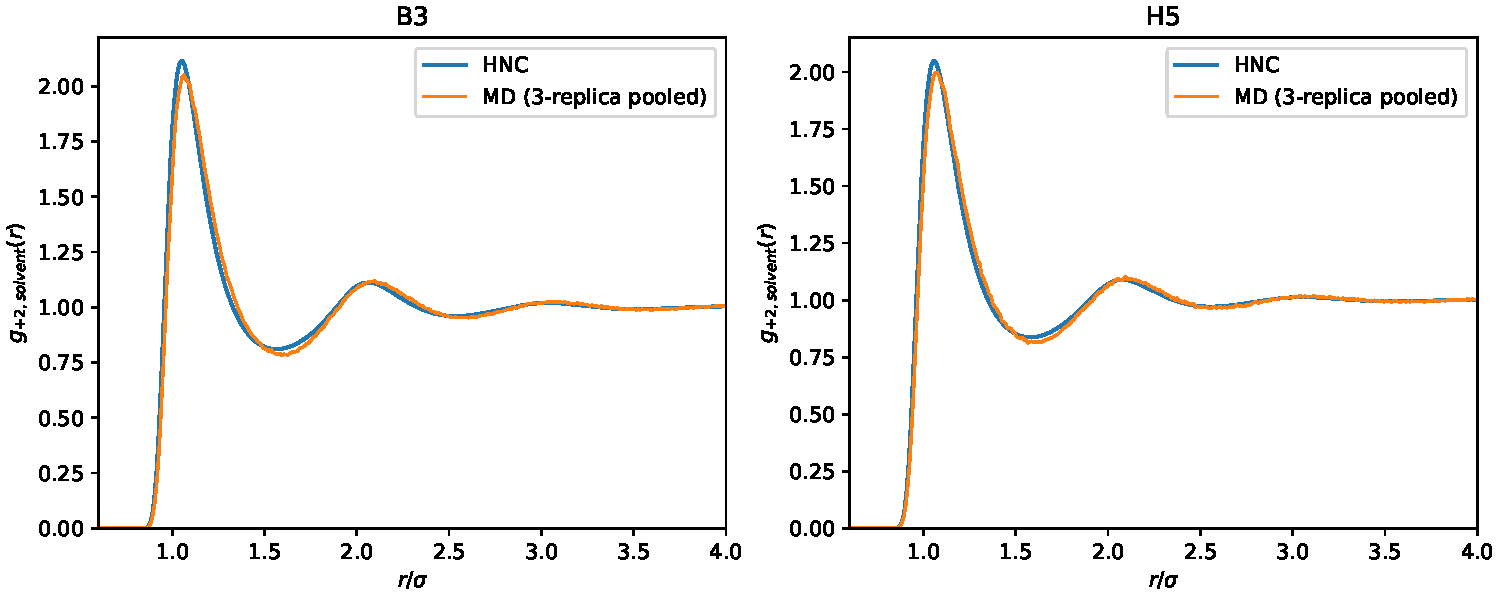
\includegraphics[width=\linewidth]{../MDPairEntropyAssessment/results/hnc_md_probe_rdf.pdf}
\caption{HNC and pooled three-replica MD radial distribution functions for a +2 probe and the primary neutral solvent in B3 and H5. Their first coordination shells agree closely, with modest differences in the first peak and minimum.}
\label{fig:pair_entropy_hnc}
\end{figure}

Table~\ref{tab:pair_entropy_contrasts} shows that pair entropy preserves most of the controlled increments: $s_2$ captures about 82\% of the U4-to-M5 increase and 79\% of the U4-to-H5 and U6-to-H7 increases. For the exact U4/L5 relabeling, both MD pair entropy and all diffusion values are identical. The pair approximation thus retains the entropy ordering, but understates the thermodynamic entropy change and leaves a composition-dependent residual (Fig.~\ref{fig:pair_entropy_benchmark}).

% Generated by generate_component_study_assets.py; do not edit numbers by hand.
\begin{table*}[t]
\centering
\caption{Paired differences in full TI excess entropy, MD pair entropy, beyond-pair residual, and the individual probe diffusivities. Entropies are per particle in $k_B$. Diffusion entries are point percent changes from paired log ratios; their nominal 95\% intervals are discussed in the text. The identical-label split is an exact mechanical null.}
\label{tab:pair_entropy_contrasts}
\small
\resizebox{\ifdim\width>\textwidth\textwidth\else\width\fi}{!}{%
\begin{tabular}{lrrrrr}
\toprule
Comparison & $\Delta s_{\rm ex}^{\rm TI}/k_B$ [95\% CI] & $\Delta s_2^{\rm MD}/k_B$ [95\% CI] & $\Delta(s_{\rm ex}-s_2)/k_B$ [95\% CI] & $\Delta D_{+2}$ & $\Delta D_{-2}$ \\
\midrule
L5/U4 & $+0.00042\;[-0.00219,+0.00304]$ & $+0.00000\;[+0.00000,+0.00000]$ & $+0.00042\;[-0.00219,+0.00304]$ & +0.0\% & +0.0\% \\
M5/U4 & $+0.03039\;[+0.02727,+0.03352]$ & $+0.02485\;[+0.02300,+0.02669]$ & $+0.00555\;[+0.00247,+0.00862]$ & +0.0\% & +2.9\% \\
H5/U4 & $+0.10322\;[+0.10209,+0.10434]$ & $+0.08170\;[+0.08077,+0.08262]$ & $+0.02152\;[+0.02057,+0.02247]$ & +3.6\% & +6.1\% \\
H7/U6 & $+0.10331\;[+0.09990,+0.10672]$ & $+0.08202\;[+0.08154,+0.08250]$ & $+0.02129\;[+0.01756,+0.02502]$ & +3.7\% & +6.6\% \\
H5/B3 & $+0.30214\;[+0.29927,+0.30501]$ & $+0.26795\;[+0.26583,+0.27007]$ & $+0.03419\;[+0.02947,+0.03891]$ & +16.8\% & +23.4\% \\
H7/B5 & $+0.30149\;[+0.29823,+0.30476]$ & $+0.26870\;[+0.26701,+0.27038]$ & $+0.03280\;[+0.03055,+0.03505]$ & +18.0\% & +17.6\% \\
B5/B3 & $-0.00320\;[-0.00543,-0.00097]$ & $-0.00312\;[-0.00545,-0.00080]$ & $-0.00008\;[-0.00387,+0.00372]$ & -1.5\% & +5.2\% \\
\bottomrule
\end{tabular}}
\end{table*}


\begin{figure}[t]
\centering
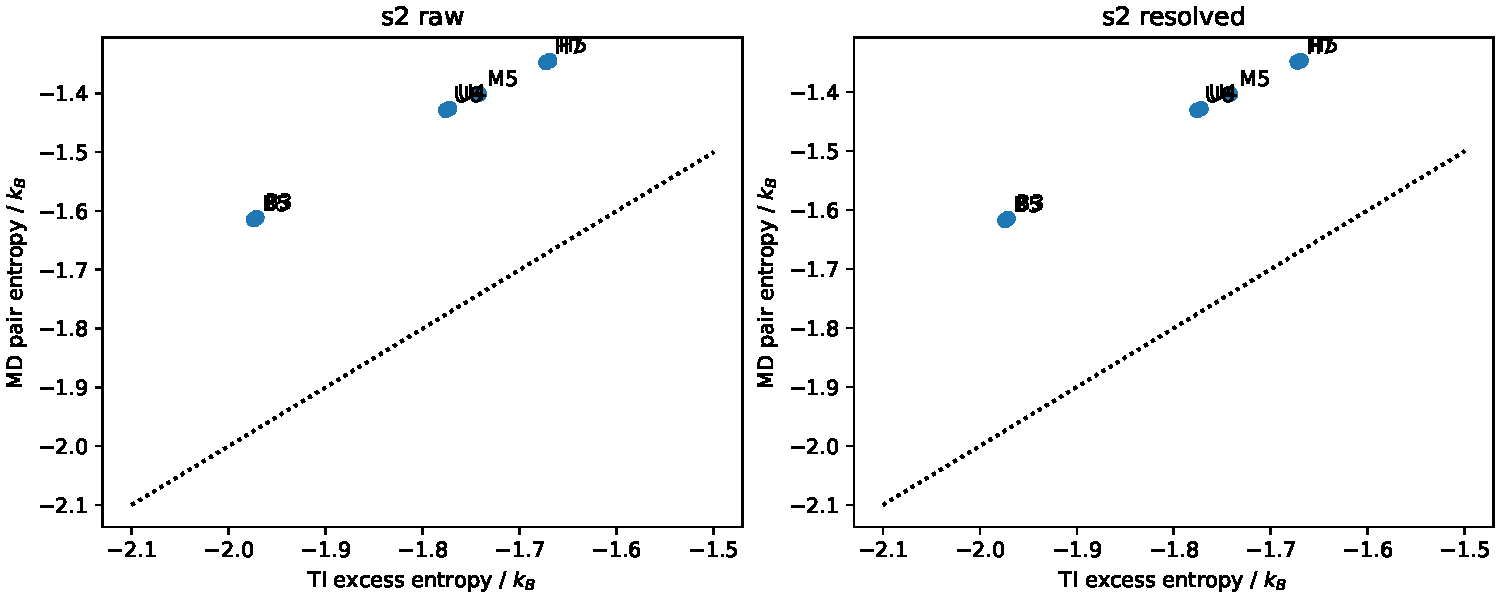
\includegraphics[width=\linewidth]{figures/component_pair_entropy_benchmark.pdf}
\caption{MD pair entropy compared with the full excess entropy from thermodynamic integration. The left panel uses the uncorrected $\Delta r=0.02$ RDF estimator; the right panel uses the resolved fine-core estimate. The dotted line denotes equality.}
\label{fig:pair_entropy_benchmark}
\end{figure}

\subsection{Label Count, Ideal Mixing, and Physical Diversification}

U4 and L5 provide an exact mechanical null. Splitting the secondary solvent into two identical labels increases the formal ideal mixing entropy by $0.30\ln2=0.20794k_B$ per particle if the labels are treated as distinguishable. Nevertheless, the diffusion coefficients are identical in every replica, and the excess-entropy difference is only $+0.00042k_B$, interval $[-0.00219,0.00304]k_B$. Component labels alone are not a mechanical driving variable for diffusion.

M5 and H5 have the same mole fractions and ideal mixing entropy as L5, but different interactions, so their entropy differences are interaction-induced excess changes. Adding monovalent salt to the baseline, B3$\to$B5, increases the ideal mixing contribution by $0.38787k_B$ but slightly \emph{lowers} the excess entropy, $\Delta s_{\rm ex}=-0.00320k_B$, interval $[-0.00543,-0.00097]k_B$. Neither mean diffusion ($+0.12\%$) nor probe diffusion ($+1.79\%$) changes significantly. More charged components therefore do not by themselves raise the excess entropy or accelerate the probes.

\subsection{Divalent-Ion Enhancement}

The largest design changes clearly increase divalent-ion mobility. H5/B3 gives $+20.05\%$, interval $[14.30,26.09]\%$, and H7/B5 gives $+17.79\%$, interval $[11.17,24.81]\%$. Both signs increase separately: $+16.8\%$ for $+2$ and $+23.4\%$ for $-2$ in H5/B3, and $+18.0\%$ and $+17.6\%$ in H7/B5, with all four paired intervals excluding zero. These comparisons also alter the mean interaction strength and local friction, so the entropy is a correlate rather than an isolated causal variable.

The controlled diversification gives a smaller response. U4$\to$H5 preserves charged composition, ionic strength, masses, nominal diameters, and mean bare pair amplitude. Mean diffusion increases by $9.47\%$, interval $[8.96,9.97]\%$, whereas probe diffusion increases by $4.81\%$, interval $[0.60,9.19]\%$. With monovalent background, U6$\to$H7 increases mean diffusion by $8.37\%$, interval $[7.31,9.44]\%$, and probe diffusion by $5.20\%$, interval $[-6.14,17.92]\%$. The moderate split raises mean diffusion by $2.99\%$ with an unresolved $1.48\%$ probe increase. The ions respond less strongly than the solvent-dominated mean.

\subsection{Rosenfeld-Like Correlation and Its Limits}

Figure~\ref{fig:new_scaling} shows a positive entropy--mobility trend for both the mean and the divalent probes. All masses, temperatures, and densities are equal, so $D_i^R=D_i\rho^{1/3}/\sqrt{T}$ differs from $D_i$ by a common constant. Unweighted fits of composition means to
\begin{equation}
\ln D_i^R=\ln A_i+B_i s_{\rm ex}/k_B
\label{eq:new_scaling}
\end{equation}
give $B_{\rm net}=0.80$ and $B_{\rm probe}=0.62$ for B3/U4/M5/H5, and $0.78$ and $0.55$ for B5/U6/H7, all with $R^2>0.99$. These fits contain only four or three composition means and do not incorporate uncertainty in both coordinates; the high $R^2$ is descriptive rather than an independent validation of a universal law. Replacing $s_{\rm ex}$ by the MD pair entropy preserves the positive trends, with $R^2$ between 0.989 and 1.000 for the mean, pooled-probe, and separate-sign fits (Fig.~\ref{fig:pair_entropy_species_diffusion}).

\begin{figure*}[t]
\centering
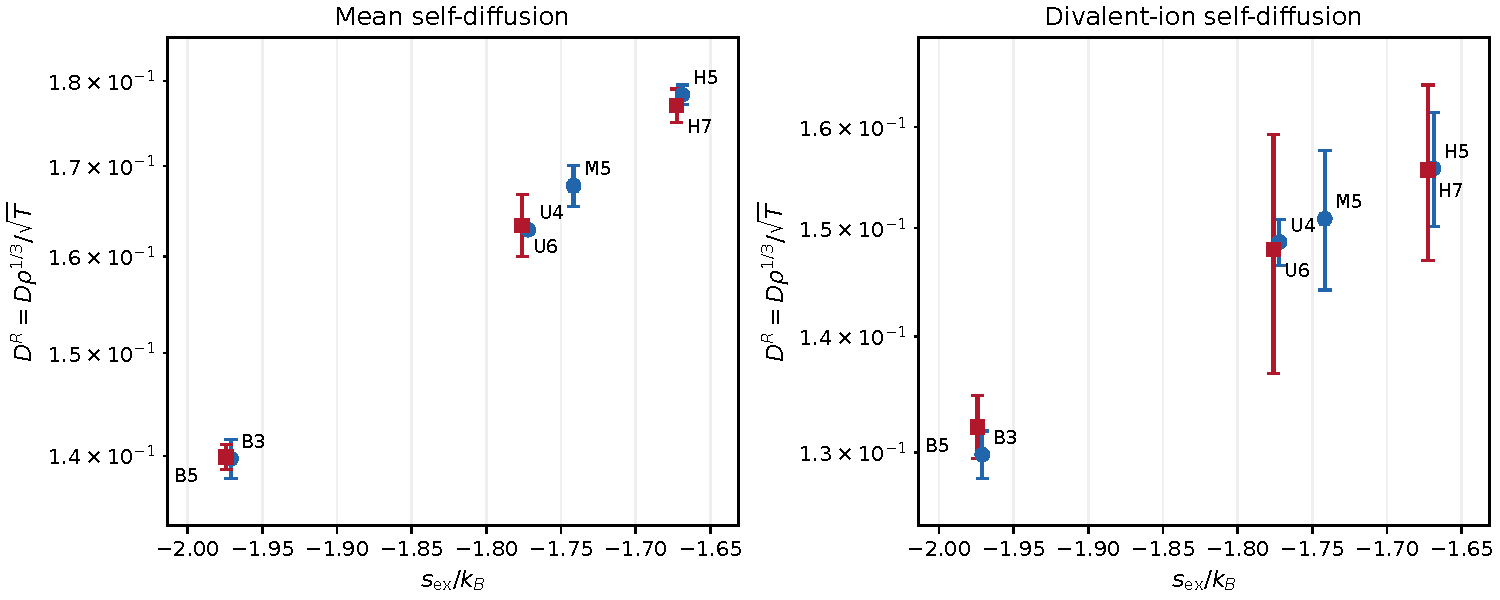
\includegraphics[width=\textwidth]{figures/component_entropy_diffusion.pdf}
\caption{Rosenfeld-reduced mean and divalent-probe self-diffusion versus MD excess entropy. Vertical axes are logarithmic. Blue circles: no monovalent background; red squares: 5\% of each monovalent sign. Bars are nominal 95\% absolute-state replica intervals. L5 coincides exactly with U4 in transport and is omitted.}
\label{fig:new_scaling}
\end{figure*}

\begin{figure*}[t]
\centering
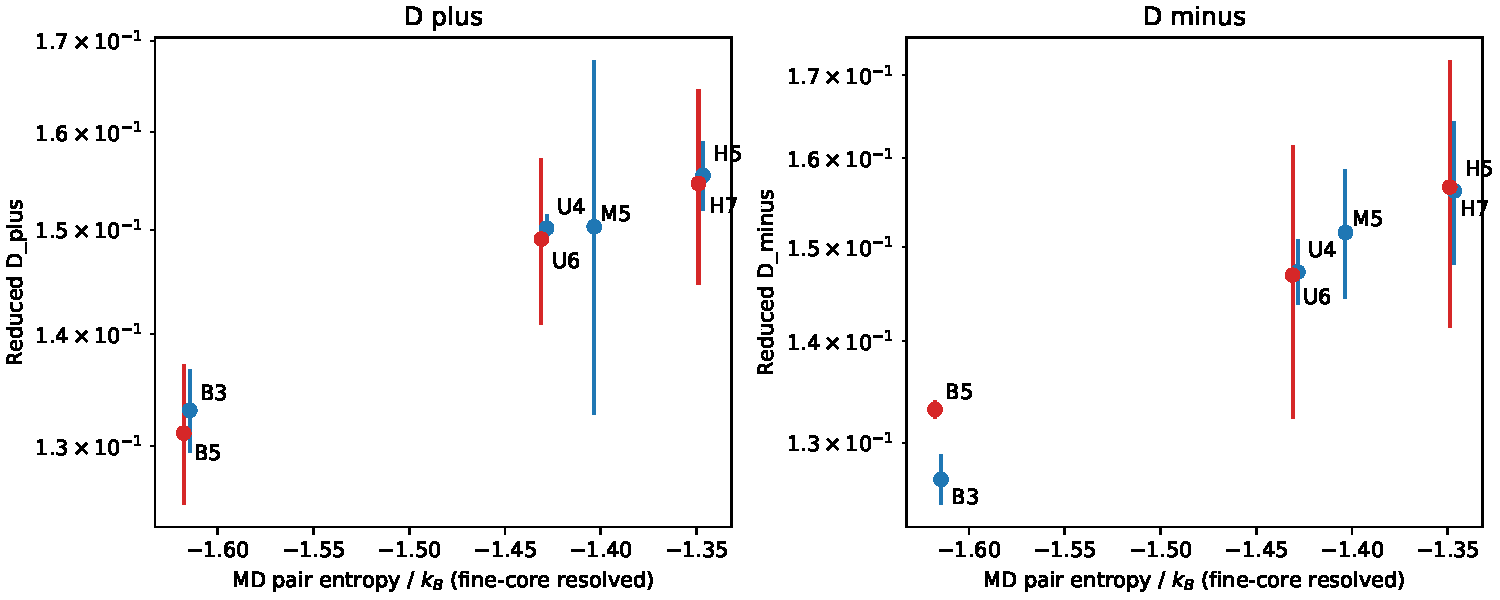
\includegraphics[width=0.92\textwidth]{figures/component_pair_entropy_species_diffusion.pdf}
\caption{Reduced self-diffusion coefficients of the +2 and $-2$ probes versus the all-species MD pair entropy. Error bars show nominal 95\% absolute-state replica intervals and exclude finite-size and estimator systematics. Blue circles: no monovalent salt; red circles: with monovalent salt. L5 is omitted because it duplicates U4 mechanically.}
\label{fig:pair_entropy_species_diffusion}
\end{figure*}

The controlled local response differs from the family fits. For H5/U4, $\Delta\ln D/\Delta(s_{\rm ex}/k_B)$ is approximately $0.88$ for the mean and $0.46$ for the probes; H7/U6 gives approximately $0.78$ and $0.49$. The probe response is thus weaker than the mean response under the same intervention. Mean self-diffusion assigns only 6\% weight to the divalent particles and cannot determine their mobility. The results support a restricted entropy--mobility association for both observables, while neither component count nor a single bulk entropy determines species mobility.

\subsection{Estimator Sensitivity and Homogeneity}
\label{sec:sensitivity}

The controlled ion point estimates remain positive, approximately 4--6\%, across the MSD windows (Table~\ref{tab:new_windows} and Fig.~\ref{fig:new_windows}), but H5/U4 loses nominal significance over 50--200$\tau$ and H7/U6 is unresolved in all three windows. The approximately 5\% ion effect is therefore a robust trend in sign but not a converged precise enhancement. VACF integrals over the final $100\tau$ support the broad mobility ordering but are too short to resolve an effect of this size independently.

% Generated by generate_component_study_assets.py; do not edit numbers by hand.
\begin{table*}[t]
\centering
\caption{Sensitivity of the paired divalent-ion diffusion change (percent) to MSD fitting window, with nominal 95\% replica intervals. The 20--100$\tau$ window is primary. The positive controlled effect is not uniformly significant across estimators/windows.}
\label{tab:new_windows}
\small
\resizebox{\ifdim\width>\textwidth\textwidth\else\width\fi}{!}{%
\begin{tabular}{lrrr}
\toprule
Comparison & 10--50$\tau$ & 20--100$\tau$ & 50--200$\tau$ \\
\midrule
H5/U4 & $+5.92\;[+1.87,+10.13]$ & $+4.81\;[+0.60,+9.19]$ & $+3.94\;[-8.44,+18.00]$ \\
H7/U6 & $+5.31\;[-1.17,+12.22]$ & $+5.20\;[-6.14,+17.92]$ & $+4.46\;[-5.66,+15.67]$ \\
\bottomrule
\end{tabular}}
\end{table*}


\begin{figure}[tb]
\centering
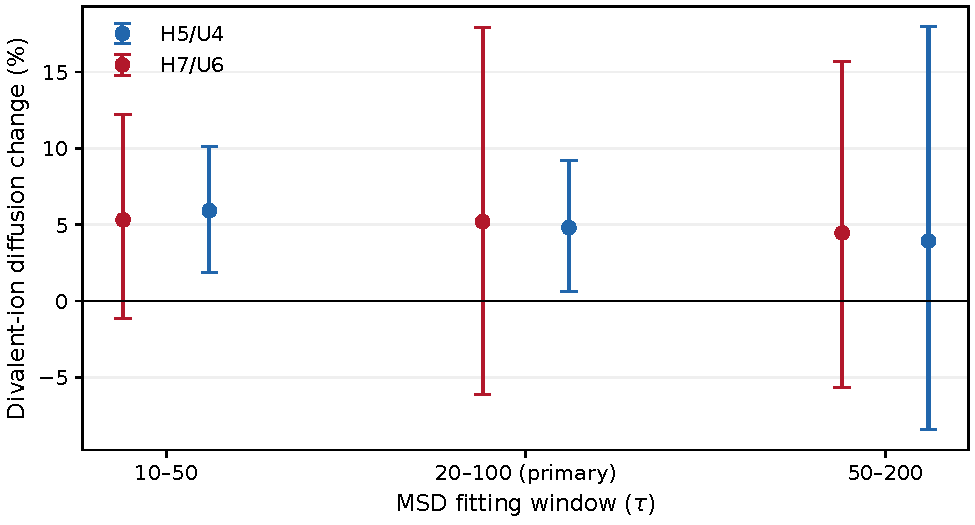
\includegraphics[width=\linewidth]{figures/component_window_sensitivity.pdf}
\caption{Controlled divalent-ion diffusion changes and nominal paired 95\% intervals for alternative MSD windows. Point estimates remain positive, but their significance depends on the window and on the monovalent background.}
\label{fig:new_windows}
\end{figure}

Charge-sign symmetry provides an additional convergence diagnostic. The B3 Hamiltonian is invariant under global charge reversal, so the long-time self-diffusion of the two probe signs must coincide. The primary-window estimate nevertheless gives $D_{+2}-D_{-2}=0.0104$, nominal replica interval $[0.0029,0.0179]$, whereas all other states have sign-difference intervals containing zero. Both probe species have identical masses and LJ parameters, random positions, one all-particle thermostat, and a common COM frame, so the asymmetry cannot be physical and must reflect finite sampling of slow ionic rearrangements, or an undetected numerical artifact. It does not affect the large baseline contrasts, for which each sign accelerates separately, but it indicates that replica intervals for single-sign diffusion of a few percent should be read as lower bounds on the uncertainty.

Switching from cubic to shape-preserving interpolation changes the dense-state entropy by at most $0.00032k_B$, and retaining all or 75\% of production instead of the final half changes it by at most $0.00165k_B$. These sensitivities are small relative to the $0.103k_B$ diversification increments, although they do not bound the error below the lowest simulated density or finite-size effects in a single box size. Low-wavevector species concentration fluctuations remain of order unity, approximately 0.48--1.80 for individual replica/species values, with no enhancement indicating incipient demixing; a single box size and the present trajectory lengths cannot exclude slower segregation.

%======================================================================
\section{Conclusions}
%======================================================================

The replicated calculations establish a positive excess-entropy--mobility association in the selected solvent-design families, with clear limits on its interpretation.
\begin{enumerate}
\item \textbf{Component count alone has no transport effect.} An exact label-only split raises the formal ideal mixing entropy while leaving diffusion identical. Monovalent salt addition slightly lowers the excess entropy and gives no resolved divalent speedup.
\item \textbf{HNC-guided interaction changes produce higher-excess-entropy, faster-ion liquids.} MD confirms entropy increases of approximately $0.30k_B$ and divalent diffusion gains of 18--20\% relative to the baselines, with both signs accelerating. HNC predicts the entropy increments to within about 7\%. These are design comparisons, not isolated entropy interventions.
\item \textbf{Controlled diversification gives a weaker ion response.} At fixed charged composition and mean bare pair amplitude, the excess entropy rises by approximately $0.103k_B$, mean diffusion by 8--9\%, and probe diffusion by approximately 5\%. The ion effect is positive in every MSD window, but its statistical significance depends on the window and is not resolved with monovalent background.
\item \textbf{Rosenfeld-like trends extend to both probe signs but do not establish a universal law.} Separate fits of $D_{+2}$ and $D_{-2}$ against either the excess entropy or the MD pair entropy have positive slopes within the selected families, while the controlled local slopes for the probes are about half those of the mean.
\item \textbf{Pair entropy captures most, but not all, of the excess entropy.} The all-species $s_2$ accounts for approximately 80\% of $s_{\rm ex}$ and of its controlled increments, leaving a composition-dependent beyond-pair residual of about $-0.32$ to $-0.36k_B$ per particle.
\end{enumerate}
Longer independent sampling and larger systems are needed to fix the size of the controlled ion response, together with the charge-sign symmetry of B3. Probe--solvent coordination, association lifetimes, and exchange kinetics, together with higher divalent concentrations and several state points at fixed composition, would test whether weaker local caging rather than a bulk entropy coordinate controls the ion mobility.

\begin{acknowledgments}
This work was supported by the Spanish Ministerio de Ciencia, Innovaci{\'o}n y Universidades and CSIC. Computational resources provided by the Scientific Computing Center at IQF-CSIC are gratefully acknowledged.
\end{acknowledgments}

\appendix
%======================================================================
\section{Two-Phase Thermodynamic Estimate of the Excess Entropy}
\label{app:2pt}
%======================================================================

The two-phase thermodynamic (2PT) method of Lin, Blanco, and Goddard~\cite{Lin2003} estimates the entropy of a liquid from the vibrational density of states, $G(\nu)$, i.e.\ the Fourier transform of the mass-weighted VACF. The spectrum is partitioned into a diffusive, gas-like component, modeled as a hard-sphere gas whose zero-frequency intensity reproduces the self-diffusion coefficient, and a solid-like remainder treated as a collection of harmonic oscillators. The gas-like fraction, or fluidicity $f$, follows from the normalized diffusivity $\Delta$, which compares the actual $G(0)$ with that of a hard-sphere gas at the same density and temperature. The entropy is then the sum of the hard-sphere-gas entropy (Carnahan--Starling) weighted by $f$ and the oscillator entropy integrated over the solid-like spectrum. Because it requires only a short trajectory, 2PT is an attractive alternative to thermodynamic integration. However, the partition is a model: the gas/solid division is not a literal population count, and for mixtures the species partial volumes entering $\Delta$ must be approximated~\cite{Lai2012}. We therefore test 2PT against the integration results of Sec.~\ref{sec:results}, rather than use it as an entropy coordinate.

We analyzed the final-$100\tau$ velocity records of all 24 replicas with a classical 2PT estimator. The spectral construction follows the revised formulation of Sun \emph{et al.}~\cite{Sun2017}, with the equal-partial-volume mixture approximation of Lai \emph{et al.}~\cite{Lai2012}: each species is assigned $\bar V_i=1/\rho$. The primary gas/solid partition exponent is $\delta=1$, and the published LJ value $\delta=1.5$ is an unfitted sensitivity. No partition, reference volume, or entropy offset is adjusted to match the integration results. The COM-corrected VACF is Gaussian-tapered with width $10\tau$, its spectrum spans the full Nyquist band and is normalized to three modes per particle, and the gas Lorentzian and its entropy tail are integrated analytically. The residual spectrum is kept signed as revised-2PT bookkeeping rather than clipped to a positive solid population.

The implementation passes analytic checks, including the fluidicity polynomial, unit invariance, a solvable VACF/Green--Kubo limit, the Lorentzian entropy tail, the dilute-gas limit, and cancellation of the classical reference and of label mixing. Mechanically identical labels give identical 2PT entropies, and state-mean probe spectral diffusivities agree with the MSD coefficients within $2.6\%$.

\begin{figure*}[t]
\centering
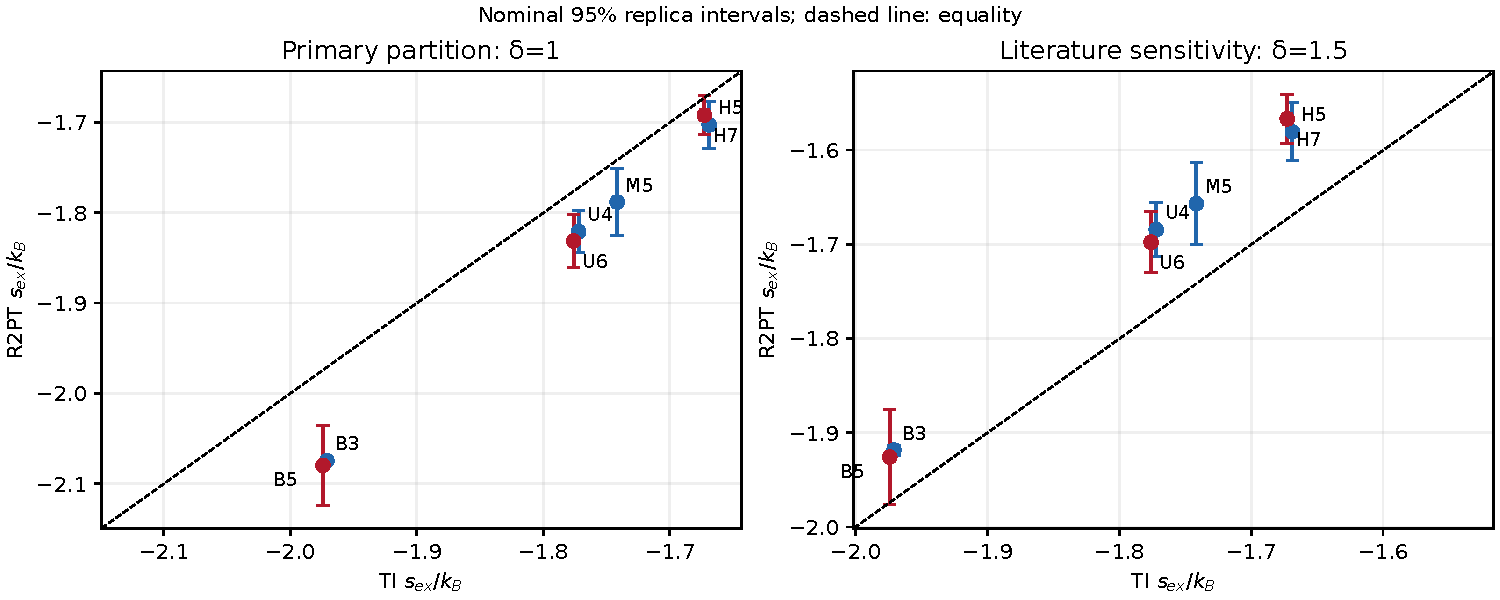
\includegraphics[width=\textwidth]{figures/component_2pt_validation.pdf}
\caption{Classical revised-2PT excess entropy against thermodynamic integration (TI) for the seven mechanically distinct mixtures. L5 duplicates U4 and is omitted. Bars are nominal 95\% absolute-state replica intervals; dashed lines denote equality. Left: primary partition $\delta=1$; right: literature sensitivity $\delta=1.5$.}
\label{fig:2pt_validation}
\end{figure*}

Internal consistency does not imply quantitative thermodynamic accuracy across compositions (Fig.~\ref{fig:2pt_validation}). For B3 the primary estimate is $-2.07445k_B$, compared with $-1.97101k_B$ from integration. The absolute biases range from about $-0.019$ to $-0.105k_B$, all with paired intervals below zero, so the error is composition dependent and comparable to the controlled entropy signal.

% Generated by generate_component_study_assets.py; do not edit numbers by hand.
\begin{table*}[t]
\centering
\caption{Controlled excess-entropy increments from TI and corrected classical revised 2PT. All entropy quantities are per particle in $k_B$. Bias is the paired difference between the 2PT and TI increments; brackets are nominal 95\% Student-$t$ intervals from three independent replica pairs (two degrees of freedom), without multiplicity correction. The primary partition is $\delta=1$; $\delta=1.5$ is an unfitted sensitivity.}
\label{tab:2pt_contrasts}
\small
\resizebox{\ifdim\width>\textwidth\textwidth\else\width\fi}{!}{%
\begin{tabular}{llrrr}
\toprule
Comparison & Partition & TI $\Delta s_{\rm ex}/k_B$ & 2PT $\Delta s_{\rm ex}/k_B$ & Bias [95\% CI] \\
\midrule
H5/U4 & $\delta=1$ & 0.10322 & 0.11818 & $+0.01496\;[-0.00544,+0.03536]$ \\
H5/U4 & $\delta=1.5$ & 0.10322 & 0.10397 & $+0.00075\;[-0.02175,+0.02326]$ \\
H7/U6 & $\delta=1$ & 0.10331 & 0.13927 & $+0.03596\;[+0.01501,+0.05692]$ \\
H7/U6 & $\delta=1.5$ & 0.10331 & 0.13086 & $+0.02755\;[+0.00705,+0.04805]$ \\
\bottomrule
\end{tabular}}
\end{table*}


For H5/U4, 2PT gives $\Delta s_{\rm ex}=0.11818k_B$ versus $0.10322k_B$ from integration (Table~\ref{tab:2pt_contrasts}), consistent within its wide interval. For H7/U6, it gives $0.13927k_B$ versus $0.10331k_B$, an overestimate of approximately $35\%$ whose bias interval excludes zero. The $\delta=1.5$ partition improves the first increment but still overestimates the second. The discrepancies survive variations of taper width, record half, frequency grid, sampling interval, and partial volume. Thermodynamic integration is therefore retained as the entropy coordinate; 2PT and the underlying VACFs remain useful dynamical diagnostics, but their species allocations are not independently measured partial molar entropies.

\begin{thebibliography}{99}

\bibitem{Rosenfeld1977}
Y. Rosenfeld,
Phys. Rev. A \textbf{15}, 2545 (1977).

\bibitem{Rosenfeld1999}
Y. Rosenfeld,
J. Phys.: Condens. Matter \textbf{11}, 5415 (1999).

\bibitem{Rosenfeld1995}
Y. Rosenfeld, E. Nardi, and Z. Zinamon,
Phys. Rev. Lett. \textbf{75}, 2490 (1995),
\href{https://doi.org/10.1103/PhysRevLett.75.2490}{doi:10.1103/PhysRevLett.75.2490}.

\bibitem{Krekelberg2009}
W.~P. Krekelberg, M.~J. Pond, G. Goel, V.~K. Shen, J.~R. Errington, and T.~M. Truskett,
Phys. Rev. E \textbf{80}, 061205 (2009),
\href{https://doi.org/10.1103/PhysRevE.80.061205}{doi:10.1103/PhysRevE.80.061205}.

\bibitem{Schmitt2025}
S. Schmitt, H. Hasse, and S. Stephan,
Nat. Commun. \textbf{16}, 2611 (2025),
\href{https://doi.org/10.1038/s41467-025-57780-z}{doi:10.1038/s41467-025-57780-z}.

\bibitem{Wang2023}
Q. Wang \textit{et al.},
Nat. Commun. \textbf{14}, 440 (2023),
\href{https://doi.org/10.1038/s41467-023-36075-1}{doi:10.1038/s41467-023-36075-1}.

\bibitem{He2026}
L. He \textit{et al.},
Mol. Syst. Des. Eng. \textbf{11}, 681 (2026),
\href{https://doi.org/10.1039/D6ME00060F}{doi:10.1039/D6ME00060F}.

\bibitem{HansenMcDonald4th}
J.-P. Hansen and I.~R. McDonald,
\textit{Theory of Simple Liquids: with Applications to Soft Matter}, 4th ed.
(Academic Press, London, 2013).

\bibitem{Morita1960}
T. Morita and K. Hiroike,
Prog. Theor. Phys. \textbf{23}, 1003 (1960),
\href{https://doi.org/10.1143/PTP.23.1003}{doi:10.1143/PTP.23.1003}.

\bibitem{Hiroike1960}
K. Hiroike,
Prog. Theor. Phys. \textbf{24}, 317 (1960),
\href{https://doi.org/10.1143/PTP.24.317}{doi:10.1143/PTP.24.317}.

\bibitem{Morita1961}
T. Morita and K. Hiroike,
Prog. Theor. Phys. \textbf{25}, 537 (1961),
\href{https://doi.org/10.1143/PTP.25.537}{doi:10.1143/PTP.25.537}.

\bibitem{Allnatt1964}
A.~R. Allnatt,
Mol. Phys. \textbf{8}, 533 (1964),
\href{https://doi.org/10.1080/00268976400100591}{doi:10.1080/00268976400100591}.

\bibitem{LombaHoye1992}
E. Lomba and J.~S. H{\o}ye,
Comput. Phys. Commun. \textbf{69}, 420 (1992),
\href{https://doi.org/10.1016/0010-4655(92)90180-7}{doi:10.1016/0010-4655(92)90180-7}.

\bibitem{Labik1985}
S. Lab{\'\i}k, A. Malijevsk{\'y}, and P. Vo{\v n}ka,
Mol. Phys. \textbf{56}, 709 (1985),
\href{https://doi.org/10.1080/00268978500102651}{doi:10.1080/00268978500102651}.

\bibitem{Kinoshita1988}
M. Kinoshita and M. Harada,
Mol. Phys. \textbf{65}, 599 (1988).

\bibitem{Singer1985}
S.~J. Singer and D. Chandler,
Mol. Phys. \textbf{55}, 621 (1985).

\bibitem{Green1952}
H.~S. Green,
\textit{The Molecular Theory of Fluids}
(North-Holland, Amsterdam, 1952).

\bibitem{Wallace1987}
D.~C. Wallace,
J. Chem. Phys. \textbf{87}, 2282 (1987).

\bibitem{Plimpton1995}
S. Plimpton,
J. Comput. Phys. \textbf{117}, 1 (1995).

\bibitem{Lin2003}
S.-T. Lin, M. Blanco, and W.~A. Goddard III,
J. Chem. Phys. \textbf{119}, 11792 (2003),
\href{https://doi.org/10.1063/1.1624057}{doi:10.1063/1.1624057}.

\bibitem{Sun2017}
T. Sun, J. Xian, H. Zhang, Z. Zhang, and Y. Zhang,
J. Chem. Phys. \textbf{147}, 194505 (2017),
\href{https://doi.org/10.1063/1.5001798}{doi:10.1063/1.5001798}.

\bibitem{Lai2012}
P.-K. Lai, C.-M. Hsieh, and S.-T. Lin,
Phys. Chem. Chem. Phys. \textbf{14}, 15206 (2012),
\href{https://doi.org/10.1039/C2CP42011B}{doi:10.1039/C2CP42011B}.

\end{thebibliography}

\end{document}
